%template1.tex
%The following LaTeX source file represents the simplest kind of slide presentation; no overlays, no included graphics. Substitute your favorite style for ``pascal''. To create the PDF file template1.pdf, (1) be sure to use the prosper class, then (2) execute the command latex template1.tex, and (3) the command dvipdf template1.dvi.

%%%%%%%%%%%%%%%%%%%%%%%%%%%%%%% template1.tex %%%%%%%%%%%%%%%%%%%%%%%%%%%%%%%%%%%
\documentclass[a4paper,blends,pdf,colorBG,slideColor]{prosper}
% definitions for slides for CSC544
% Lutz Hamel, (c) 2007

\hypersetup{pdfpagemode=FullScreen}

\usepackage{amssymb}
\usepackage{latexsym}
\usepackage{amsmath}
%\usepackage[usenames]{color}
\usepackage{xypic}


\newcommand{\term}[1]{\ensuremath{\mbox{\bf #1}}}
\newcommand{\nonterm}[1]{\ensuremath{\mbox{#1}}}
\newcommand{\ifstmt}[3]{\ensuremath{{\bf if}\; {#1}\;{\bf then}\;{#2}\;{\bf else}\;{#3}\;\term{end}}}
\newcommand{\whilestmt}[2]{\ensuremath{{\bf while}\; {#1}\;{\bf do}\;{#2}\; \term{end}}}
\newcommand{\funcstmt}[3]{\ensuremath{{\bf fun}\; {#1}\; {\bf is}\; {#2} \; {\bf return}\; {#3}}}
\newcommand{\syntaxset}[1]{\ensuremath{\mbox{\bf #1}}}
\newcommand{\orbar}{\;|\;}
\newcommand{\bs}[1]{\begin{slide}{#1}\ptsize{8}}
\newcommand{\es}{\end{slide}}
\newcommand{\co}{\,\colon\;}
\newcommand{\pair}[2]{\ensuremath{\langle {#1}, {#2} \rangle}}
\newcommand{\encode}[1]{\ensuremath{\langle {#1} \rangle}}
\newcommand{\mytab}{\makebox[.15in]{}}
%\newcommand{\abs}[1]{{\mid{#1}\mid}}
\newcommand{\abs}[1]{{|{#1}|}}
\newcommand{\ol}[1]{\overline{#1}}

\newcommand{\qaccept}{\ensuremath{q_{\mbox{\tiny accept}}}}
\newcommand{\qreject}{\ensuremath{q_{\mbox{\tiny reject}}}}
\newcommand{\accept}{{\em accept}}
\newcommand{\reject}{{\em reject}}

\newcommand{\machine}[1]{
	\begin{quote}
	{#1}
	\end{quote}
	}

\newcommand{\fdef}[1]{
	\begin{center}
	\fbox{
	\begin{minipage}{3.5in}
	{\bf Definition:}
	{#1}
	\end{minipage}
	}
	\end{center}
	}

\newcommand{\ftheorem}[1]{
	\begin{center}
	\fbox{
	\begin{minipage}{3.5in}
	{\bf Theorem:}
	{#1}
	\end{minipage}
	}
	\end{center}
	}

\newcommand{\flemma}[1]{
	\begin{center}
	\fbox{
	\begin{minipage}{3.5in}
	{\bf Lemma:}
	{#1}
	\end{minipage}
	}
	\end{center}
	}


\newcommand{\fframe}[1]{
	\begin{center}
	\fbox{
	\begin{minipage}{3.5in}
	{#1}
	\end{minipage}
	}
	\end{center}
	}

\newcommand{\nframe}[1]{
	\begin{center}
	\begin{minipage}{3.5in}
	{#1}
	\end{minipage}
	\end{center}
	}

\begin{document}


\bs{Generators vs. Recognizers}
Up to now we have only described languages in terms of machines that
{\bf recognize} a particular language.  

But we could also imagine describing a language by a system that is able to
{\bf generate} all the strings in a language.

\begin{center}
    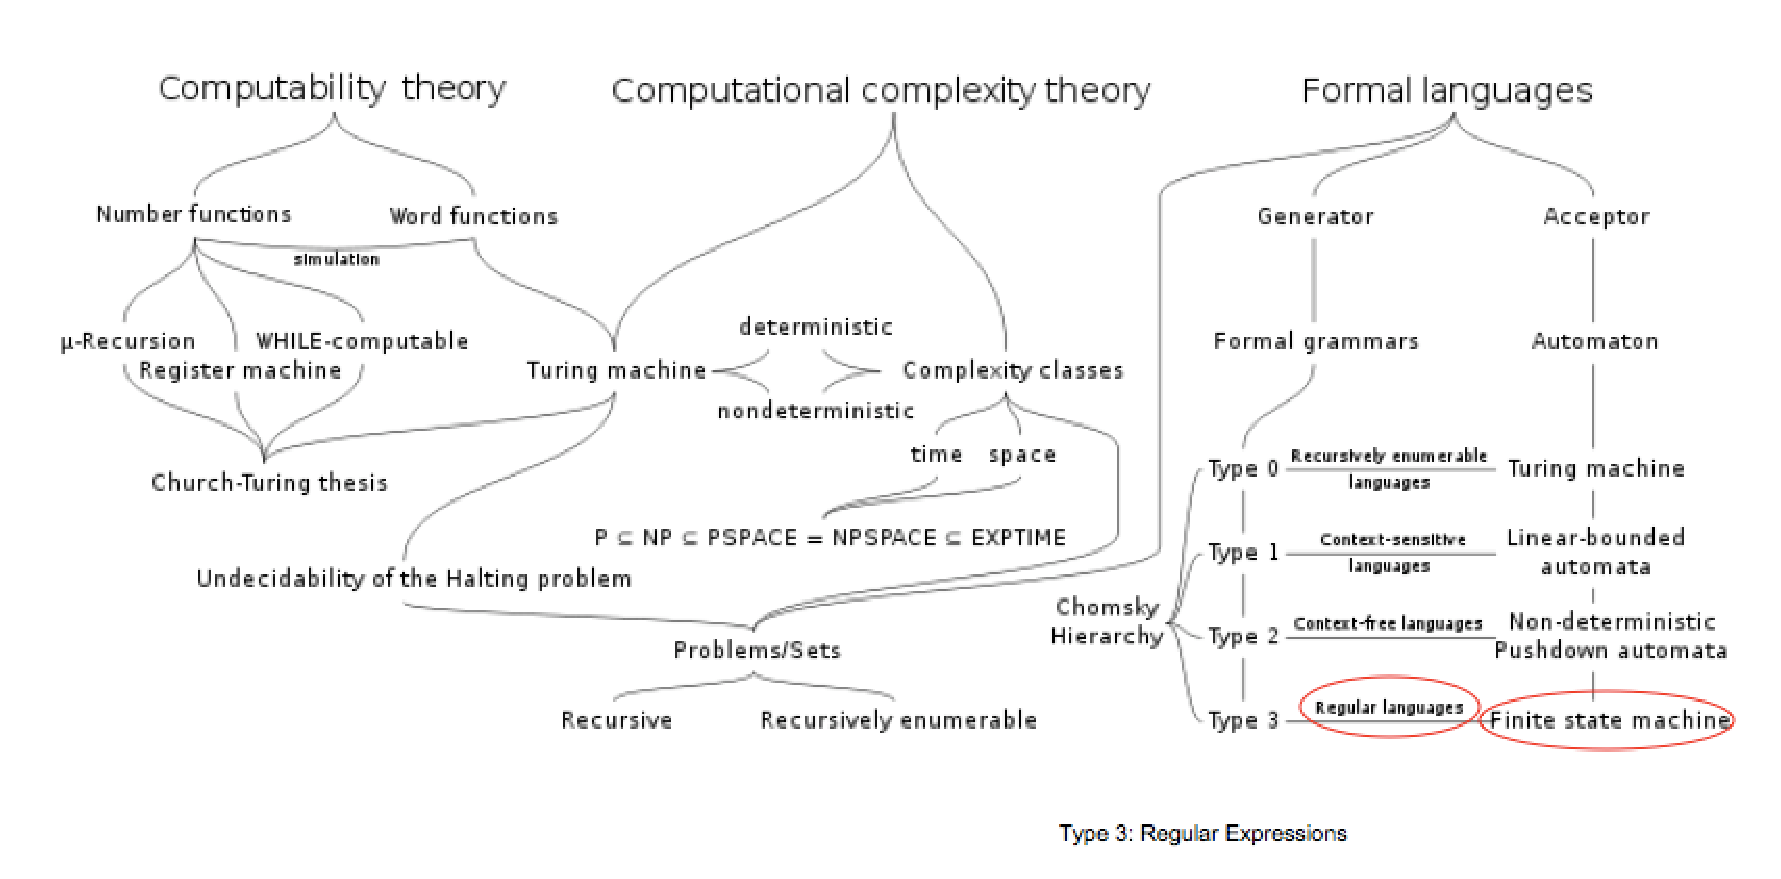
\includegraphics[height=45mm]{images/course-road-map-02.eps}
\end{center}

\es

\bs{Rewriting Systems}

In order to define a system that generates a language we introduce a new model
of computation: Rewriting Systems.

Informally, a rewriting system consists of an alphabet and a set of rules over that alphabet.

You are already familiar with a very powerful rewriting system: Algebra!

Here, the alphabet are the numerals and variable names in addition to operator names.
The rules consist of your standard algebraic laws.

\es

\bs{Rewriting Systems}

{\bf Example:} Consider the set of algebraic laws:
\begin{eqnarray}
x + x &=& 2 \times x\\
y + 0 &=& y\\
x + y &=& y + x
\end{eqnarray}

We can apply these rules to strings formed from the alphabet.  Consider:
\[
\begin{array}{rcll}
5 + 3 + 5 + 0 &=& 5 + 3 + 5 & \mbox{(rule 2)}\\
	&=& 5 + 5 + 3& \mbox{(rule 3)}\\
	&=& 2 \times 5 + 3& \mbox{(rule 1)}
\end{array}
\]

The string that we start with is called the {\bf input string} and the string that we end up with is called 
the {\bf normal form} because no other rules apply to this final string.

For our purposes we introduce a special rewriting system called a {\bf String Rewriting System}.
\es


\bs{String Rewriting Systems}

\vspace{.1in}
{\bf Definition:} [String Rewriting System (SRS)]  A {\em string rewriting system} is a tuple $(\Sigma,R)$ where,
\begin{itemize}
\item $\Sigma$ is a finite {\em alphabet} where $\Sigma^*$ is the set of (possibly empty) strings over $\Sigma$.\footnote{The set $\Sigma^*$ is a convenient short hand to describe all the strings over the alphabet $\Sigma$.}
\item $R$ is a binary relation on $\Sigma^*$, i.e., $R\subseteq \Sigma^*\times\Sigma^*$. Each element  
$(u,v)\in R$ is called a rewriting rule and is usually written as $u \rightarrow v$.
\end{itemize}

\vspace{.1in}
An inference step in this formal system is: given a string $u$ and a rule $u \rightarrow v$ with $u,v \in \Sigma^*$ and
$u \rightarrow v \in R$ then the string $u$ can be {\em rewritten} as the string $v$.

\vspace{1in}
\es


\bs{String Rewriting Systems}

\small
In order for an SRS $(\Sigma,R)$ to be useful we allow rules to be applied to substrings of given strings; let $s = xuy$,$t=xvy$, and $u\rightarrow v \in R$ with $x,y,u,v \in \Sigma^*$, then we say that {\em $s$ rewrites to $t$} and we write,
\[
s \Rightarrow t.
\]
More formally,

\vspace{.1in}
{\bf Definition:} [one-step rewriting relation] Let $(\Sigma,R)$ be a string rewriting system,
then the {\em one-step rewriting relation} $RW$ is defined as the set $\Sigma^*\times\Sigma^*$ with $s\Rightarrow t \in RW$ for strings $s,t \in\Sigma^*$
 if and only if there exist $x, y, u, v \in\Sigma^*$ such that $s = xuy, t = xvy$, and $u\rightarrow v \in R$.

\vspace{.1in}
In plain English: any two string $s,t$ belong to the relation $RW$ if and only if they can be related by 
a rewrite rule in the rule set $R$.

\vspace{.1in}
{\bf Exercise:} $R \subseteq RW$.  Why? (spoiler alert, next page holds the solution)
\es

\bs{String Rewriting Systems}

{\bf Proposition:} $R \subseteq RW$.

\vspace{.1in}

{\bf Proof:} We use the definition of a subset, $R \subseteq RW \mbox{ iff } \forall e\in R.\, e\in RW$, for our proof.
There is nothing to prove for the `only if' direction. More interesting is the `if' direction, if we can show that all elements of $R$ are 
also elements of $RW$ then it follows from the definition that $R \subseteq RW$. 

\vspace{.1in}
An element of $R$ is the pair $(u,v)$ with $u,v\in \Sigma^*$ if the rewriting system contains the rule $u\rightarrow v$.
An element of $RW$ is the pair $(xuy,xvy)$ with $u,v,x,y\in \Sigma^*$ if the rewriting system contains the rule
$u \rightarrow v$.  Thus, $RW$ contains pairs of strings where the first string contains a substring that is the left side
of a rule in the rewriting system.  Observe that $(u,v)\in RW$ with $x$ and $y$ the empty strings.  It follows that
all elements of $R$ are members of $RW$.$\Box$


\es

\bs{String Rewriting Systems}

\small
Given a string rewriting system $(\Sigma,R)$, we can obviously apply the rewriting rules to the results of a rewriting step.  This gives
rise to {\em derivations}
\[
s_n \Rightarrow s_{n-1} \Rightarrow\ldots \Rightarrow s_1 \Rightarrow s_0,
\]
with $s_k \in \Sigma^*$.

\vspace{.1in}
We say that $s_0$ is a {\em normal form} if $s_0$ cannot be rewritten any further.

\vspace{.1in}
The {\em transitive closure} $\Rightarrow^*$ of the one-step rewriting relation is the set all pairs of strings that are related
to each other via zero or more rewriting steps, e.g.,
\[
s_n \Rightarrow^* s_0,
\]
and
\[
s_i \Rightarrow^* s_i.
\]

\es

\bs{String Rewriting Systems}

\small

{\bf Example:} The urn game.  An urn contains black and white beads.  The game has the following rules:
{\scriptsize
\begin{itemize}
\item if you remove two black beads you have to replace them with a black bead.
\item if you remove two white beads you have to replace them with a black bead.
\item if you remove a white and a black bead you have to replace them with a white bead.
\end{itemize}
}
Given the contents of an urn, what is the outcome of the game?

\vspace{.1in}
The game can be set up as a string rewriting system $(\Sigma,R)$.
 Let $\Sigma = \{ \mbox{black}, \mbox{white} \}$ and let $R$ be the following set of rules,
\[
\begin{array}{rcl}
\mbox{black black} &\rightarrow& \mbox{black}\\
\mbox{white white} &\rightarrow& \mbox{black}\\
\mbox{black white} &\rightarrow& \mbox{white}\\
\mbox{white black} &\rightarrow& \mbox{white}
\end{array}
\]

{\scriptsize
\[
\mbox{black white black white} \Rightarrow \mbox{black white white} \Rightarrow \mbox{white white} \Rightarrow \mbox{black}
\]
\[
\mbox{black black white white} \Rightarrow \mbox{black white white} \Rightarrow \mbox{white white} \Rightarrow \mbox{black}
\]
\[
\mbox{black black white} \Rightarrow \mbox{black white} \Rightarrow \mbox{white}
\]
\[
\mbox{black white black} \Rightarrow \mbox{black white} \Rightarrow \mbox{white}
\]
}
\es


\bs{String Rewriting Systems}

\small
{\bf Observations:} 
\begin{itemize}
\item It can be shown that for each urn there exists a unique normal form, the order of rule application does not 
matter.
\item If we interpret a rewrite rule $u \rightarrow v$ as specifying that {\em $u$ is the same as $v$} then we can 
interpret the normal form as a 'value' for an urn. Consider,
\[
\mbox{black white black} \Rightarrow \mbox{black white} \Rightarrow \mbox{white},
\]
the normal form 'white' can be considered the value for the urn.
\item We say that two urns are equivalent if they have the same normal form,

{\scriptsize
\[
\xymatrix{
\mbox{black white black} \ar@{=>}[rd]^{*} &\equiv &\mbox{black black white}\ar@{=>}[ld]_{*}  \\
&\mbox{white}&
}
\]
}
\end{itemize}
\es

\bs{String Rewriting Systems}

\small
{\bf Example:} Palindrome generator.  We construct a string rewriting system $(\Sigma,R)$ with
$\Sigma = \{a,b,\ldots,z, \alpha\}$ and $R$ the set of rules,
\[
\begin{array}{rcl}
\alpha & \rightarrow & a \alpha a\\
\alpha & \rightarrow & b \alpha b\\
& \vdots&\\
\alpha &\rightarrow& z \alpha z\\
a\alpha a & \rightarrow & a\\
b\alpha b & \rightarrow & b\\
& \vdots&\\
z\alpha z & \rightarrow & z\\
\alpha &\rightarrow& \epsilon
\end{array}
\]
\vspace{.1in}
\[
\alpha \Rightarrow r \alpha r \Rightarrow r a \alpha a r \Rightarrow r a d \alpha d a r \Rightarrow r a d a r
\]
{\bf Exercise:} Derive the normal form: $racecar$

{\bf Exercise:} Derive the normal form: $redder$

\es


\bs{Grammars}

\small
{\bf Observations:}
\begin{itemize}
\item We have seen in the case of the palindrome generator that SRSs are well suited for generating strings with 
structure.
\item By modifying the standard SRS just slightly we obtain a convenient framework for generating strings
with desirable structure -- {\em Grammars}
\end{itemize}

\vspace{.2in}

{\bf Definition:} [Grammar] A {\em grammar} is a 4-tuple $(V,\Sigma,R,s)$ such that,
\begin{itemize}
\item $V$ is a set of variables called the {\em non-terminals},
\item $\Sigma$ with $V\cap \Sigma = \emptyset$,  is a set of symbols called the {\em terminals},\footnote{The fact that $V$ and $\Sigma$ are non-overlapping means
that there will never be confusion between terminals and non-terminals.}
\item $R$ is a set of rules of the form $u \rightarrow v$ with $u,v\in(V\cup \Sigma)^*$,\footnote{All sets in this definition
are considered to be {\em finite}.}
\item $s$ is called the {\em start symbol} and $s\in V$.
\end{itemize}
\es

\bs{Grammars}

\small
{\bf Example:} Grammar for arithmetic expressions.  We define the grammar $(V,\Sigma, R, s)$ as follows:
\begin{itemize}
\item $V = \{ E \}$,
\item $\Sigma = \{ a, b, c, +, *, (, )\}$,
\item $R$ is the set of rules,
{\scriptsize
\[
\begin{array}{rcl}
E & \rightarrow & E + E \\
E & \rightarrow & E * E \\
E & \rightarrow & ( E )\\
E & \rightarrow & a\\
E & \rightarrow & b\\
E & \rightarrow & c
\end{array}
\]
}
\item $s = E$ (clearly this satisfies $s\in V$).
\end{itemize}
With grammars,derivations always start with the start symbol. Consider,
\[
E\Rightarrow E * E \Rightarrow ( E ) * E \Rightarrow ( E + E ) * E \Rightarrow (a + E) * E \Rightarrow (a + b) * E
\Rightarrow (a + b) * c.
\]
Here, $(a+b)*c$ is a normal form often also called a {\em terminal} or {\em derived string}.

\es

\bs{Grammars}

{\bf Exercise:} Identify the rule that was applied at each rewrite step in the above derivation.

{\bf Exercise:} Derive the string $((a))$.

{\bf Exercise:} Derive the string $a + b * c$.  

\es

\bs{Grammars}

\small
{\bf Example:} Grammar for strings of a's and b's with at least one b in them.  We define the grammar $(V,\Sigma, R, s)$ as follows:
\begin{itemize}
\item $V = \{ S,A,B \}$,
\item $\Sigma = \{ a, b\}$,
\item $R$ is the set of rules,
{\scriptsize
\[
\begin{array}{rcl}
S & \rightarrow & A\, b \, B\\
A & \rightarrow & \epsilon\\
A & \rightarrow & a\, A\\
A & \rightarrow & b\, A\\
B & \rightarrow & \epsilon\\
B & \rightarrow & a\, B\\
B & \rightarrow & b\, B
\end{array}
\]
}
\item $s = S$.
\end{itemize}

{\bf Exercise:} Derive string aba.

{\bf Exercise:} Derive string bbb.

{\bf Exercise:} Derive string b.

\es


\bs{Grammars}

\small
We are now in the position to define exactly what we mean by the {\em language of a grammar}.

\vspace{.2in}
{\bf Definition:}[Language of a Grammar] Let $G = (V,\Sigma,R,s)$ be a grammar, then we define the {\em language of
grammar $G$} as the set of all terminal strings that can be derived from the start symbol $s$ by rewriting
using the rules in $R$.  Formally,
\[
L(G) = \{ q \mid s \Rightarrow^* q \wedge q\in \Sigma^*\}.
\]

\vspace{.3in}
{\bf Example:} Let $J = (V,\Sigma,R,s)$ be the grammar of Java, then $L(J)$ is the set of all possible Java 
programs.
\es


\bs{Grammars}

\small
{\bf Observations:}  
\begin{itemize}
\item With the concept of a language we can now ask interesting questions.  For example,
given a grammar $G = (V,\Sigma,R,s)$ and some sentence $p\in \Sigma^*$, does $p$ belong to $L(G)$?
\item If we let $J$ be the grammar of Java, then asking whether some string $p\in \Sigma^*$ is in $L(J)$
is equivalent to asking whether $p$ is a {\em syntactically correct program}.
\item We can prove language membership by by showing that the 
sentence $p$ in question can be derived from the start symbol.  Graphically, 
{\scriptsize
\[
\xymatrix{
s \ar@{=>}[rd]^{*} &\equiv &p\ar@{=>}[ld]_{*}  \\
&p&
}
\]
}

\end{itemize}

\es


\bs{Grammars}

{\bf Observations:} 
\begin{itemize}
\item By restricting the shape of the rewrite rules in a grammar we obtain different language {\em classes}.
\item  The most famous set of language classes is the {\em Chomsky Hierarchy}.
\end{itemize}
\es

\bs{\Large The Chomsky Hierarchy}

\scriptsize
%{\bf The Chomsky Hierarchy:}
Let $G = (V,\Sigma,R,s)$ be a grammar.  Restricting the shape of the rules in $R$ gives rise to the following hierarchy.

\begin{table*}[htdp]
%\caption{The Chomsky Hierarchy}
\begin{center}
{\tiny
\begin{tabular}{|c|c|c|c|}
Rules & Grammar & Language & Machine \\ \hline
$\alpha \rightarrow \beta$ & Type-0 & Recursively Enumerable & Turing machine \\
$\alpha A \beta \rightarrow \alpha\gamma\beta$  & Type-1 & Context-sensitive & Linear-bounded Turing machine\\
$A  \rightarrow \gamma$  & Type-2 & Context-free & Pushdown automaton\\
$A \rightarrow a$ and $A \rightarrow a B$ & Type-3 & Regular & Finite state automaton
\end{tabular}
}
\end{center}
\label{default}
\end{table*}%
where $\alpha,\beta,\gamma\in (V \cup \Sigma)^*, A,B \in V, a\in \Sigma$.
In Type-1 $\gamma$ is not allowed to be the empty string.

\vspace{.1in}
\begin{center}
    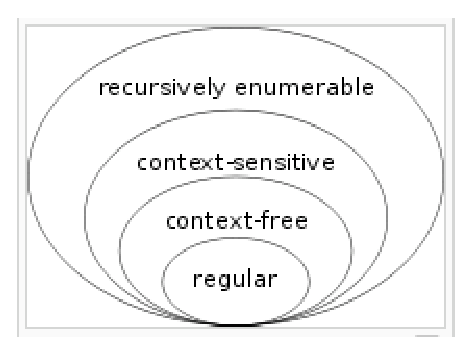
\includegraphics[height=30mm,width=35mm]{images/chomsky-hierarchy}
\end{center}


\es



\bs{\large Type 3: Regular Grammars}

A grammar $G = (V,\Sigma,R,s)$ is called regular (type 3) if and only if the rules in $R$ are of the form
\footnote{If the language include the empty string then the rule $s \rightarrow \epsilon$ will need to be added 
to the grammar.} 
\[
A \rightarrow a\, B
\]
or 
\[
A \rightarrow a
\]
with $A,B \in V$ and $a\in\Sigma$.
\es

\bs{\large Type 3: Regular Grammars}

{\bf Example:} Grammar for strings of one or more 1's followed by a single 0.  We define the grammar $(V,\Sigma, R, s)$ as follows:
\begin{itemize}
\item $V = \{ A,S \}$,
\item $\Sigma = \{ 0, 1\}$,
\item $R$ is the set of rules,
{\scriptsize
\[
\begin{array}{rcl}
S & \rightarrow & 1\, A \\
A & \rightarrow & 1\, A \\
A & \rightarrow & 0
\end{array}
\]
}
\item $s = S$.
\end{itemize}

\es

\bs{\large Type 3: Regular Grammars}

\small
{\bf Example:} Grammar for strings of a's and b's with at least one b in them.  We define the grammar $(V,\Sigma, R, s)$ as follows:
\begin{itemize}
\item $V = \{ A,B \}$,
\item $\Sigma = \{ a, b\}$,
\item $R$ is the set of rules,
{\scriptsize
\[
\begin{array}{rcl}
A & \rightarrow & a\, A \\
 A & \rightarrow &b\, A \\
A & \rightarrow &  b\,B \\
A & \rightarrow &   b\\
B & \rightarrow & a\, B \\
B & \rightarrow &b\, B \\
B & \rightarrow & a \\
B & \rightarrow &  b
\end{array}
\]
}
\item $s = A$.
\end{itemize}

This shows that the language of strings of a's and b's with at least one b in them is a regular language.
\es

\bs{\large Regular Languages and Regular Grammars}

\fframe{{\bf Lemma:} If a language is recognized by a FA then it is generated by a type-3 grammar.}

{\bf Proof:} We show that if a language is recognized by a DFA then we can construct a type-3
grammar that generates it.
Let $M=(Q,\Sigma,\delta,q_0,F)$ be a DFA that recognizes language $L(M)$.
We now construct the type-3 grammar
$G = (V,\Sigma,R, s)$ that simulates the computations of the DFA :
\begin{itemize}
\item For each state $q\in Q$ we construct the non-terminal symbol $\langle q \rangle\in V$, 
\item The terminal set $\Sigma$ in the grammar  is the same as the alphabet of the machine,
\item We construct the rule set $R$ as follows, let $q,p\in Q$ and let $a\in\Sigma$,
\begin{itemize}
 \item add a  rule of the form $\langle q\rangle \rightarrow  a\, \langle p\rangle$ for each transition  $\delta(q, a) = p$,
\item add a rule of the form $\langle q\rangle \rightarrow  a$ for each transition $\delta(q, a) = p$ where $p\in F$,
\item add a rule of the form $\langle q_0\rangle \rightarrow \epsilon$   if the initial state is an accepting state, i.e., $q_0\in F$.
\end{itemize}
\item We let $s = \langle q_0 \rangle$.
\end{itemize}
\es

\bs{\large Regular Languages and Regular Grammars}

Now,for any string $w=w_1 w_2\ldots w_n\in L(M)$ the machine $M$ will perform the computation
\[
q_0 w_1 w_2 \ldots w_n \vdash  w_1 q_1 w_2 \ldots w_n \vdash  \ldots  \vdash 
 w_1 w_2 \ldots q_{n-1}w_n \vdash  w_1 w_2 \ldots w_n q_n
\]
with $q_n \in F$. We can show by induction on $n$ that the input string is generated by the grammar with the derivation
\[
\langle q_0\rangle \Rightarrow w_1\langle q_1\rangle \Rightarrow w_1 w_2\langle q_2 \rangle \Rightarrow \ldots 
\Rightarrow w_1 w_2 \ldots w_{n-1} \langle q_{n-1}\rangle \Rightarrow w_1 w_2 \ldots w_{n-1} w_n  
\]

\es

\bs{\large Regular Languages and Regular Grammars}
\scriptsize
Consider:
\begin{enumerate}
\item $s=\epsilon$ -- in the machine this gives rise to the computation $q_0$ which is also an accepting state, the grammar derives the empty string via the rule $\langle q_0\rangle \rightarrow \epsilon$.
\item $s=w_1$ -- this gives rise to the computation $q_0 w_1 \vdash  w_1 q_1$ where $q_1$ is an accepting state;
the grammar derives string $w_1$ via the rule $\langle q_0\rangle \rightarrow  w_1$.
\item Any substring $s=w_1 w_2\ldots w_k$ of string $w=w_1 w_2\ldots w_n\in L(M)$ with $k \le n$-- then the machine performs the computation
\[
q_0 w_1 w_2 \ldots w_n \vdash  w_1 q_1 w_2 \ldots w_n \vdash  \ldots  \vdash 
 w_1 w_2 \ldots q_{k-1}w_k \vdash  w_1 w_2 \ldots w_k q_k
\]
where $q_k$ might or might not be an accepting state;
as inductive hypothesis
we assume that the grammar derives the string $w_1 w_2 \ldots w_{k-1}$ with the following derivation
\[
\langle q_0\rangle \Rightarrow w_1\langle q_1\rangle \Rightarrow w_1 w_2\langle q_2 \rangle \Rightarrow \ldots 
\Rightarrow w_1 w_2 \ldots w_{k-1} \langle q_{k-1}\rangle 
\]
then it follows from the inductive hypothesis and the fact that by construction there has to exist at least one of the
following rules
\[
\langle q_{k-1}\rangle \rightarrow w_k
\]
if $q_k$ is an accepting state or
\[
\langle q_{k-1}\rangle \rightarrow w_k\langle q_{k}\rangle
\]
if not,
that the grammar can generate the string $s=w_1 w_2\ldots w_k$.
\end{enumerate}
$\Box$
\es

\bs{\large Regular Languages and Regular Grammars}

\fframe{{\bf Lemma:}  if a language  is generated by a type-3 grammar then it is recognized by a FA.}

{\bf Proof:} We show that if a language is generated by a type-3 grammar then it is recognized by a DFA.
Let $G =(V,\Sigma,R,s)$ be a type-3 grammar, then we construct the machine $M = (Q,\Sigma,\delta,q_0,F)$
as follows,
\begin{itemize}
\item For each $A \in V$ in grammar $G$ we construct the state $q_A\in Q$ in machine $M$,
\item The terminal set $\Sigma$ in $G$ becomes the alphabet $\Sigma$ for the machine,
\item Construct the transition function $\delta$ as follows,
\begin{itemize}
\item for each rule of the form $A \rightarrow a\, B \in R$ we construct the transition $\delta(q_A,a) = q_B$,
\item for each rule of the form $A \rightarrow a \in R$ we construct the transition $\delta(q_A,a) = q_F$ with
$q_F \in F$,
\item for each rule of the form $A \rightarrow \epsilon \in R$ we add the state $q_A$ to the set of accepting states, F.
\end{itemize}
\item the initial state $q_s = q_0$.
\end{itemize}

\es

\bs{\large Regular Languages and Regular Grammars}

Now,for any string $w=w_1 w_2\ldots w_n\in L(G)$, we can show by induction that a derivation in $G$,
\[
\langle q_0\rangle \Rightarrow w_1\langle q_1\rangle \Rightarrow w_1 w_2\langle q_2 \rangle \Rightarrow \ldots 
\Rightarrow w_1 w_2 \ldots w_{n-1} \langle q_{n-1}\rangle \Rightarrow w_1 w_2 \ldots w_{n-1} w_n  
\]
has an equivalent computation for the machine $M$,
the machine $M$ will perform the computation,
\[
q_0 w_1 w_2 \ldots w_n \vdash  w_1 q_1 w_2 \ldots w_n \vdash  \ldots  \vdash 
 w_1 w_2 \ldots q_{n-1}w_n \vdash  w_1 w_2 \ldots w_n q_n
\]
with $q_n \in F$. 
$\Box$.
\es

\bs{\large Regular Languages and Regular Grammars}

\fframe{{\bf Theorem:} A language is recognized by a FA if  and only if it is generated by a type-3 grammar.}

{\bf Proof:} Follows directly from the two previous lemmas.
\es

\bs{Regular Expressions}

As you might have noticed, regular grammars are a little awkward to construct.  There is a another
generator for regular languages called {\em regular expressions}.
\es

\bs{Regular Expressions}
\begin{center}
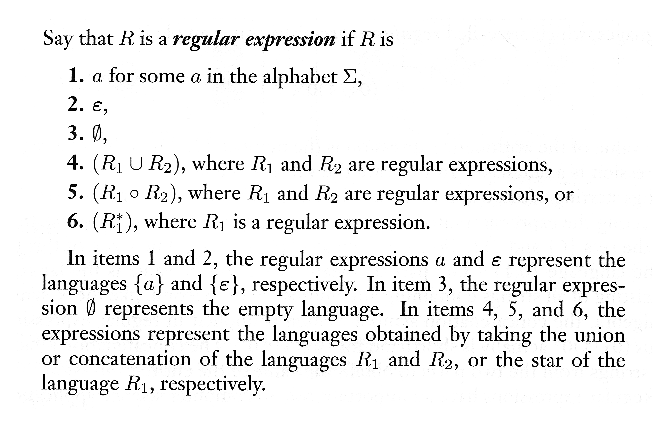
\includegraphics[height=55mm]{images/reg-exp-def.eps}
\end{center}
\es

\bs{Regular Expressions}
\begin{center}
\includegraphics[height=70mm]{images/reg-exp-example.eps}
\end{center}
\es

\bs{\large Regular Languages and Regular Expressions}
\vspace{.2in}
\begin{center}
\fframe{{\bf Theorem:} A language is regular if and only if a regular expression generates it.}
\end{center}
\vspace{.2in}
{\bf Proof Sketch:}\footnote{A formal proof of this appears in the book; pp66ff 1st \& 2nd eds.} Let $L$ be some language.
\begin{description}
\item[If $L$ is regular, then a regular expression generates it.] If $L$ is regular then some FA recognizes it.  For every FA we can construct an equivalent regular
expression.
\item[If some regular expression generates $L$, then it is a regular language.] For every
regular expression that generates $L$ we can construct an equivalent FA that
recognizes $L$.
\end{description}
\vspace{.5in}
\es

\bs{Regular Grammars and Expressions}

\fframe{
{\bf Corollary:} Regular Grammars and Regular Expressions generate the same class of languages.
}

Follows immediately from the previous two theorems.
\es


\end{document}
%%%%%%%%%%%%%%%%%%%%%%%%%%% end of template1.tex %%%%%%%%%%%%%%%%%%%%%%%%%%%%%%%%

